\documentclass[11pt,a4paper]{article}
\usepackage[utf8]{inputenc}
\usepackage[T1]{fontenc}
\usepackage{graphicx}
\usepackage{listings}
\usepackage{xcolor}
\usepackage{hyperref}
\usepackage{amsmath}
\usepackage{amssymb}
\usepackage{tikz}
\usepackage{geometry}
\usetikzlibrary{arrows.meta,positioning,fit}
\geometry{margin=1in}

\definecolor{codegreen}{rgb}{0,0.6,0}
\definecolor{codegray}{rgb}{0.5,0.5,0.5}
\definecolor{codepurple}{rgb}{0.58,0,0.82}
\definecolor{backcolour}{rgb}{0.95,0.95,0.92}

\lstdefinestyle{coursestyle}{
    backgroundcolor=\color{backcolour},
    commentstyle=\color{codegreen},
    keywordstyle=\color{magenta},
    numberstyle=\tiny\color{codegray},
    stringstyle=\color{codepurple},
    basicstyle=\ttfamily\small,
    breakatwhitespace=false,
    breaklines=true,
    captionpos=b,
    keepspaces=true,
    numbers=left,
    numbersep=5pt,
    showspaces=false,
    showstringspaces=false,
    showtabs=false,
    tabsize=2
}

\lstset{style=coursestyle}

\title{IREE Advanced:\\
Architecture, Compilation Pipeline, and Runtime}
\author{Djordje Todorovic}
\date{March 2026}

\begin{document}

\maketitle

\tableofcontents
\newpage

\section{Introduction and Architecture Overview}

\subsection{IREE in the Machine Learning Compiler Ecosystem}

When we train a neural network using a framework such as PyTorch, we work at a very high level of abstraction. We write Python code that defines layers and logic, while PyTorch handles the complexity of actually executing these operations on hardware. However, when it is time to execute the model--whether on a mobile device, an embedded system, or some custom hardware--we face a central challenge: how do we transform our high-level model into efficient executable code that can run across different hardware targets?

The answer to this is IREE, the Intermediate Representation Execution Environment. IREE is a compiler and runtime system designed specifically to bridge the gap between high-level machine learning models and the wide range of hardware platforms on which those models need to run. As you learned in previous lessons, the compilation journey typically flows from PyTorch through Torch-MLIR, which converts PyTorch models into MLIR representations. IREE then takes over from that point: it accepts MLIR input and performs transformations that produce executable code tailored to specific hardware targets.

Recall from the MLIR lessons that MLIR provides a flexible, extensible infrastructure for representing programs at multiple levels of abstraction. IREE uses exactly this MLIR foundation to implement its multi-dialect compilation flow. Roughly speaking, the complete compilation flow therefore looks like this:

\begin{quote}
PyTorch \(\rightarrow\) Torch-MLIR \(\rightarrow\) IREE \(\rightarrow\) executable code.
\end{quote}

The output of IREE is a portable bytecode format that can be loaded and executed by the IREE runtime system on the target device.

But why do we need IREE when other machine learning model compilation systems, such as TVM, which you studied earlier, already exist? To answer this question, we need to understand the unique challenges of deploying machine learning models across different hardware environments and see what makes IREE's approach and design distinct.

\section{IREE Design Philosophy}

Machine learning model execution presents a set of requirements that traditional compilers were not designed to handle. Unlike general-purpose programs, machine learning models have special characteristics: they operate primarily on large tensors, they exhibit regular computation patterns that can benefit from specialized optimizations, and they must achieve high performance across a diverse range of hardware, from GPUs to resource-constrained mobile processors.

IREE is designed around several main principles that make it distinctive: portability, performance, multi-device execution, and progressive lowering through multiple levels of abstraction.

\subsection{Portability}

Portability is perhaps IREE's most recognizable feature, and it is important to understand exactly what that means. IREE provides portability at the source level: you write the model once at a high level, for example in PyTorch or JAX, and can then compile it for many different hardware targets.

What makes IREE portable is that the entire compilation process--from the high-level model to hardware-specific code--uses the same compiler infrastructure and follows the same flow regardless of the target hardware. IREE achieves this through a carefully designed Hardware Abstraction Layer, or HAL, which provides a uniform interface for compiling toward a variety of devices. During compilation, the HAL dialect represents operations in a target-independent way; only in the final code generation phase does hardware-specific code appear. Whether the target is a CPU through LLVM, an NVIDIA GPU through CUDA, an AMD GPU through ROCm, a mobile GPU through Vulkan or Metal, or even a custom accelerator, IREE follows the same compilation stages.

In short: write once, compile for each target, deploy everywhere. IREE removes the need to rewrite the model for different hardware, but you still need to compile separately for each kind of device you want to support. This matters because it means that hardware vendors can add support for new accelerators by implementing only a HAL driver and a code generation backend, without changing the rest of the compilation flow or the models themselves.

For this course, we will focus exclusively on the CPU backend, which uses LLVM to generate optimized machine code. Although IREE supports many other targets--including Vulkan for cross-platform GPU execution, CUDA for NVIDIA GPUs, ROCm for AMD GPUs, Metal for Apple devices, and even VMVX, a portable virtual machine with vector extensions--the CPU backend provides an excellent foundation for understanding IREE's compilation model. The principles we learn for CPU code generation largely transfer to other backends, although each backend has its own specific optimizations and considerations.

\subsection{Performance}

Performance is equally critical. Machine learning inference must be fast in order to be useful in production systems. IREE achieves high performance through aggressive optimization at multiple levels. It does not simply translate operations one by one from the input. Instead, it performs sophisticated analyses to understand the structure of the computation and applies transformations such as operation fusion, where multiple operations are combined to reduce memory traffic; tiling, where large operations are broken into pieces whose sizes are suitable for cache memory; and vectorization, where operations are mapped to SIMD instructions for parallel execution.

These optimizations are not generic. They are carefully tuned based on the characteristics of the target hardware and the structure of the input program. Evidence that IREE can be genuinely high-performing can be seen in AMD's contribution to the MLPerf Inference benchmark suite in 2024, where AMD used IREE to implement Stable Diffusion XL (SDXL) for its MI325X accelerators, demonstrating that IREE can achieve competitive performance. This benchmark is especially significant because MLPerf is an industry-standard benchmark suite. See the SDXL benchmark software overview in AMD's ROCm blog: \href{https://rocm.blogs.amd.com/artificial-intelligence/mi325x-accelerates-mlperf-inference/README.html#sdxl-benchmark-software-overview}{MI325X Accelerates MLPerf Inference}.

\subsection{Multi-Device Execution}

The third principle, multi-device execution, addresses the reality that modern ML deployments often involve heterogeneous hardware configurations. A single system may contain CPUs, GPUs, and specialized accelerators, each with different strengths. IREE supports partitioning a model across multiple devices, allowing different parts of the computation to execute on the hardware best suited for them.

For example, certain operations may run on the CPU while others execute on the GPU, with IREE managing data transfers and synchronization between devices. This heterogeneous execution capability becomes increasingly important as hardware ecosystems become more diverse and specialized.

\subsection{Progressive Lowering}

The fourth principle, progressive lowering, is central to how IREE is structured. Instead of trying to compile directly from high-level operations to machine code in one enormous step, IREE defines a series of intermediate dialects, each of which represents the program at a different level of abstraction. The compilation process passes through these dialects in stages, with each stage performing transformations appropriate for its abstraction level.

This multi-level approach has several advantages. It allows optimizations to be cleanly separated by responsibility: high-level optimizations such as fusion happen early, while low-level optimizations such as register allocation happen later. It also makes the compiler more modular and easier to understand, extend, and debug.

\section{The Multi-Dialect Compilation Pipeline}

\begin{figure}[htbp]
\centering
\resizebox{0.98\textwidth}{!}{%
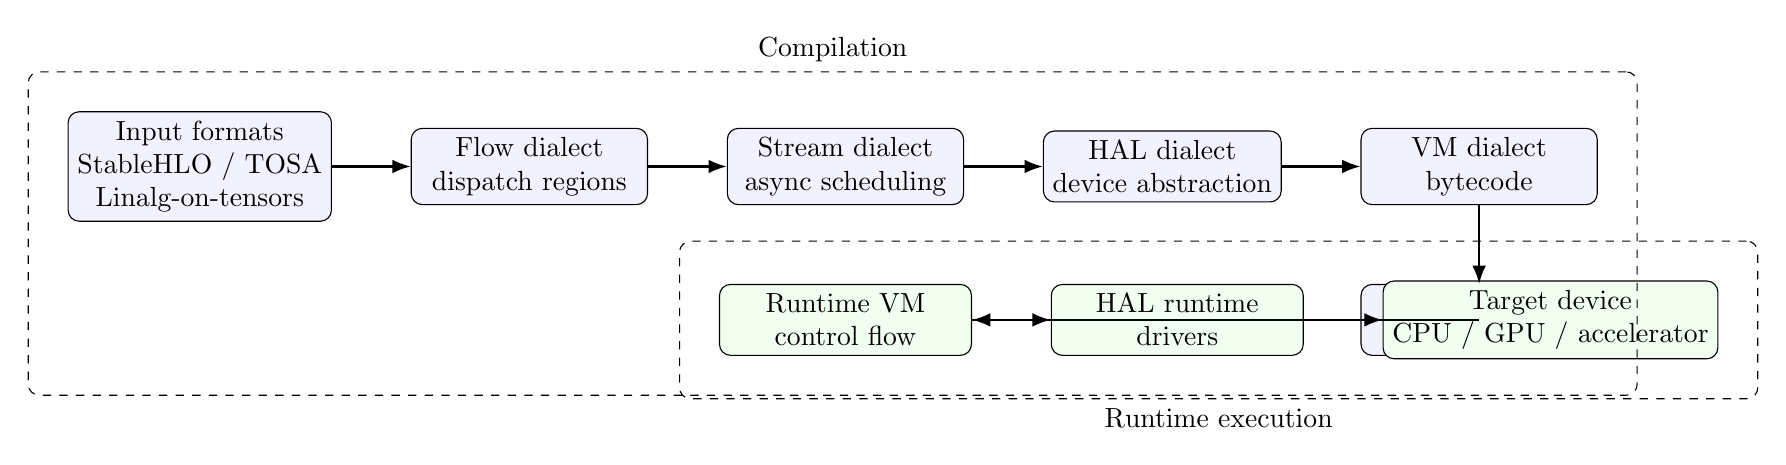
\begin{tikzpicture}[
  node distance=10mm and 10mm,
  box/.style={draw, rounded corners, align=center, minimum width=30mm, minimum height=9mm, fill=blue!5},
  runtimebox/.style={draw, rounded corners, align=center, minimum width=32mm, minimum height=9mm, fill=green!6},
  arrow/.style={-Latex, thick},
  group/.style={draw, dashed, rounded corners, inner sep=5mm}
]
\node[box] (inputs) {Input formats\\StableHLO / TOSA\\Linalg-on-tensors};
\node[box, right=of inputs] (flow) {Flow dialect\\dispatch regions};
\node[box, right=of flow] (stream) {Stream dialect\\async scheduling};
\node[box, right=of stream] (hal) {HAL dialect\\device abstraction};
\node[box, right=of hal] (vm) {VM dialect\\bytecode};
\node[box, below=of vm] (vmfb) {\texttt{.vmfb}\\VM FlatBuffer};

\node[runtimebox, below=of stream] (runtimevm) {Runtime VM\\control flow};
\node[runtimebox, right=of runtimevm] (runtimehal) {HAL runtime\\drivers};
\node[runtimebox, right=of runtimehal] (device) {Target device\\CPU / GPU / accelerator};

\draw[arrow] (inputs) -- (flow);
\draw[arrow] (flow) -- (stream);
\draw[arrow] (stream) -- (hal);
\draw[arrow] (hal) -- (vm);
\draw[arrow] (vm) -- (vmfb);
\draw[arrow] (vmfb) |- (runtimevm);
\draw[arrow] (runtimevm) -- (runtimehal);
\draw[arrow] (runtimehal) -- (device);

\node[group, fit=(inputs) (flow) (stream) (hal) (vm) (vmfb), label={[align=center]above:Compilation}] {};
\node[group, fit=(runtimevm) (runtimehal) (device), label={[align=center]below:Runtime execution}] {};
\end{tikzpicture}
}
\caption{High-level IREE architecture, showing the multi-dialect compilation pipeline and runtime system. The diagram illustrates progressive lowering from input formats through the Flow, Stream, HAL, and VM dialects to executable bytecode, as well as how the runtime components work together to execute the compiled module.}
\end{figure}

This figure shows the architecture of IREE, providing a visual map of the compilation and execution processes that we will explore in detail. Notice how the compilation side progressively transforms the program through several dialect stages, while the runtime side provides the infrastructure for execution. Understanding this pipeline is essential for working with IREE, whether we are simply compiling models or developing compiler support for a new kind of hardware.

The journey begins with the input representation. IREE accepts several input formats, including StableHLO, which is often used for models from JAX and TensorFlow; TOSA, the Tensor Operator Set Architecture used by TensorFlow Lite; and Linalg-on-tensors, a dialect within MLIR that represents linear algebra operations over multidimensional tensors. Regardless of the input format, IREE's first task is to convert this input into a form suitable for further processing. This conversion may include canonicalization, where operations are put into a standard form; dimension inference, where the compiler determines the sizes of intermediate results; and constant folding, where expressions that can be executed at compile time are evaluated immediately.

\subsection{Flow Dialect}

Once the input has been processed, compilation enters the Flow dialect stage. The Flow dialect is where IREE makes decisions about how to partition operations. Machine learning models often consist of long sequences of operations, and executing each operation individually would be inefficient because of the cost of memory reads and writes.

The Flow dialect introduces the concept of dispatch regions, which represent groups of operations that will be executed together as one unit. The compiler analyzes data dependencies between operations and determines which operations can be fused into the same dispatch region. The Flow dialect performs transformations at a high level of abstraction, where we think about transformations over whole tensors rather than over individual elements.

\subsection{Stream Dialect}

After the Flow dialect has partitioned operations, compilation continues toward the Stream dialect. While Flow groups work that can be performed together, Stream decides when and where that work should be performed.

The Stream dialect introduces the concept of asynchronous execution. On modern hardware, especially GPUs and accelerators, we often want to overlap computation with data transfers and hide latency. The Stream dialect makes scheduling decisions, determines when resources such as memory buffers should be allocated and deallocated, and inserts synchronization operations to ensure that data dependencies are respected. The output of the Stream dialect is a representation that explicitly models the asynchronous nature of execution on modern hardware.

\subsection{HAL Dialect}

Next comes the HAL dialect, the Hardware Abstraction Layer. This is where IREE's portability comes into focus. The HAL dialect provides a uniform representation of hardware operations that is independent of any specific device. It introduces concepts such as devices, which represent compute units; buffers, which represent memory regions; command buffers, which are sequences of operations to execute; and executables, which represent compiled code that can run on the final device.

The HAL dialect is target-independent. The same HAL representation can be compiled for a CPU, GPU, or another accelerator.

\subsection{The Device-Host Model}

An important concept underlying HAL is the device-host model, a fundamental paradigm in heterogeneous computing. It is important to understand that, during execution, the program always begins running on some CPU. The term ``host'' refers to that CPU, which runs the main program--in IREE's case, the VM bytecode--while ``device'' refers to the target hardware. That device may be a GPU, DSP, neural processing unit, or even a separate CPU optimized for compute-intensive work.

The host is responsible for control flow, orchestrating overall execution, and managing resources. The device is responsible for executing the actual compute kernels: the dispatch regions that contain the heavy numerical work. The host prepares data, sends work to the device, manages synchronization, and processes results. HAL abstracts this device-host interaction, providing a uniform interface regardless of whether the device is actually a separate GPU or simply a set of optimized CPU threads.

\subsection{Code Generation}

Within the HAL compilation phase, target-specific code generation takes place. This is where we encounter the term \emph{codegen}, short for code generation. Codegen refers to the process of translating higher-level operations into lower-level instructions executable by specific hardware. In traditional compilers, codegen is the backend phase that produces assembly or machine code. In IREE, codegen is invoked during the HAL phase and is responsible for taking the abstract dispatch regions created in the Flow dialect and generating efficient, hardware-specific implementations of those regions.

\subsection{VM Dialect}

The final compilation stage is the VM dialect. This dialect represents the program as bytecode that can be executed by the IREE runtime environment. The VM dialect is a low-level, register-based representation that includes instructions for function calls, control flow, arithmetic operations, and interaction with HAL to execute compiled kernels.

The output of the VM compilation stage is a serialized bytecode module saved in a file with the \texttt{.vmfb} extension, which stands for VM FlatBuffer. This bytecode module is portable across different machines with the same target assumptions and can be loaded and executed by the IREE runtime.

\section{Understanding the IREE Runtime System}

In the previous section, we focused primarily on the program compilation flow, but it is equally important to understand the runtime system that executes the compiled bytecode. The IREE runtime is what brings our compiled models to life, providing the infrastructure needed to load a module, manage resources, and execute computations on real hardware. The runtime has a two-layer architecture: the VM, or Virtual Machine, on top, and HAL, the Hardware Abstraction Layer, underneath.

The VM is a bytecode interpreter/compiler, similar in concept to the Java Virtual Machine or the Python interpreter, but specifically designed for machine learning workloads. When we load a \texttt{.vmfb} file into the runtime, the VM reads the bytecode and sets up the execution environment. The VM manages the program's control flow--handling function calls, loops, and conditional branches--and maintains program state, including variables and intermediate results. One key design decision in IREE is that the VM itself is hardware-agnostic. It does not know whether it is running on a CPU, GPU, or another accelerator. This decision keeps the VM simple and portable.

So how does the VM actually execute compute work on hardware? This is where the HAL runtime enters the picture. When the VM encounters an instruction to execute a dispatch, corresponding to one of the dispatch regions created during compilation, it delegates that work to HAL. The HAL runtime provides a device abstraction that encapsulates all hardware-specific details. Each hardware backend implements the HAL interface: there is a HAL implementation for CPUs, one for CUDA GPUs, one for Vulkan, and so on. In short, HAL is the layer responsible for connecting and enabling interaction between the host and the device.

This two-layer runtime architecture--VM on top, HAL underneath--provides a clean separation between portable execution logic and hardware-specific behavior. The VM can remain simple and maintainable because it does not handle the complexity of different hardware platforms. HAL can be optimized for each backend, with each implementation using the unique capabilities of its target hardware. At the same time, the HAL interface ensures that the VM sees a consistent execution model regardless of the hardware. This is what allows IREE to achieve write-once-run-anywhere portability without sacrificing performance.

\section{IREE Repository Structure}

Before we dive deeper into the compilation and execution flow in the following sections, it is useful to have a mental map of how the IREE project is organized. The IREE repository is large and contains many components, but its structure follows the organization below.

\subsection{Compiler Infrastructure: \texttt{compiler/}}

The \texttt{compiler} directory contains all infrastructure needed to compile models. The main source code lives under \texttt{compiler/src/iree/compiler/}, with several important subdirectories.

\subsubsection{Dialects: \texttt{Dialect/}}

The \texttt{Dialect/} directory contains definitions of IREE MLIR dialects:

\begin{itemize}
    \item \texttt{Dialect/Flow/}: workload partitioning and dispatch region formation.
    \item \texttt{Dialect/Stream/}: scheduling and asynchronous execution.
    \item \texttt{Dialect/HAL/}: Hardware Abstraction Layer operations.
    \item \texttt{Dialect/VM/}: virtual machine bytecode operations.
    \item \texttt{Dialect/Util/}: common utility operations.
\end{itemize}

Each dialect subdirectory contains files that define operations, types, and transformations specific to that dialect.

\subsubsection{Code Generation: \texttt{Codegen/}}

The \texttt{Codegen/} directory contains source code for generating code for target hardware:

\begin{itemize}
    \item \texttt{Codegen/LLVMCPU/}: CPU code generation using LLVM, which is our primary focus.
    \item \texttt{Codegen/LLVMGPU/}: GPU code generation for CUDA and ROCm.
    \item \texttt{Codegen/SPIRV/}: Vulkan/SPIR-V code generation.
    \item \texttt{Codegen/Common/}: shared utilities across backends.
\end{itemize}

\subsubsection{Other Key Directories}

\begin{itemize}
    \item \texttt{InputConversion/}: preprocessing that happens before the Flow dialect.
    \item \texttt{Pipelines/}: orchestration of the overall compilation flow.
    \item \texttt{GlobalOptimization/}: whole-program optimization.
    \item \texttt{DispatchCreation/}: logic for forming dispatch regions.
\end{itemize}

\subsection{Runtime System: \texttt{runtime/}}

The runtime directory, \texttt{runtime/src/iree/}, contains the execution engine.

\subsubsection{Virtual Machine: \texttt{vm/}}

The \texttt{vm/} directory contains the implementation of the bytecode interpreter:

\begin{itemize}
    \item \texttt{vm/bytecode/}: bytecode execution engine.
    \item module loading, context management, and invocation support.
\end{itemize}

\subsubsection{Hardware Abstraction Layer: \texttt{hal/}}

The \texttt{hal/} directory contains the runtime device abstraction:

\begin{itemize}
    \item \texttt{hal/drivers/local\_task/}: multi-threaded CPU driver for production performance.
    \item \texttt{hal/drivers/local\_sync/}: single-threaded CPU driver for debugging.
    \item \texttt{hal/drivers/cuda/}: NVIDIA GPU driver.
    \item \texttt{hal/drivers/vulkan/}: Vulkan GPU driver.
    \item \texttt{hal/drivers/metal/}: Apple GPU driver.
\end{itemize}

The HAL runtime provides a uniform interface to all of these diverse hardware backends.

\subsection{Tools and Utilities: \texttt{tools/}}

The \texttt{tools/} directory contains command-line utilities for working with IREE:

\begin{itemize}
    \item \texttt{iree-compile}: the main compiler tool, from input to \texttt{.vmfb}.
    \item \texttt{iree-run-module}: loads and executes compiled modules.
    \item \texttt{iree-opt}: tests individual passes and inspects IR transformations.
    \item \texttt{iree-benchmark-module}: performance measurement tool.
\end{itemize}

We will use some of these tools extensively throughout this course.

\subsection{Tests and Examples}

\begin{itemize}
    \item \texttt{tests/}: test cases organized by compilation stage and functionality.
    \item \texttt{tests/e2e/}: end-to-end model tests.
    \item \texttt{samples/}: example programs demonstrating IREE capabilities.
\end{itemize}

These are excellent resources when learning about specific features.

\section{Summary}

In this section, we established the context for understanding IREE. We saw where IREE fits into the machine learning model deployment pipeline, understood its core design principles, and gained a high-level overview of its compilation and execution process. We also became familiar with the structure of the IREE repository.

In the following sections, we will go deeper into each compilation stage, examining the specific transformations that happen in the Flow, Stream, HAL, and VM dialects. We will also look more deeply at the runtime architecture that executes compiled code. Before all of that, however, we need to set up our development environment, which is the topic of the next section.

\end{document}
